\documentclass[tikz,border=8pt]{standalone}
% Shared look for every TikZ diagram. Load with \input{../../tools/tikz-style.tex}
\usepackage[sfdefault]{roboto}
\usetikzlibrary{arrows.meta, positioning, shapes.geometric, calc, fit, backgrounds}
\definecolor{cblue}{HTML}{4C78A8}
\definecolor{corange}{HTML}{F58518}
\definecolor{cgreen}{HTML}{54A24B}
\definecolor{cred}{HTML}{E45756}
\definecolor{cpurple}{HTML}{B279A2}
\definecolor{cgrey}{HTML}{6B6B6B}
\tikzset{
  every picture/.style={font=\sffamily, line width=1.2pt},
  box/.style={draw=#1, fill=#1!12, rounded corners=4pt, align=center, inner sep=7pt, minimum height=1.1cm},
  box/.default=cgrey,
  arrow/.style={-{Stealth[length=3mm]}, draw=cgrey, line width=1.4pt},
  title/.style={font=\sffamily\bfseries\Large},
  note/.style={font=\sffamily\small, text=cgrey, align=center},
}
\AtBeginDocument{\hyphenpenalty=10000 \exhyphenpenalty=10000}

% Left: the front at time T and at T + dt, a distance F dt apart; T climbs dt over F dt, so its steepest slope is 1/F.
% Right: fast marching at S's 0.1 m cell (fmm_anim.py, gridplan.fmm): the neighbour across (right) was reached at
% a = 3.0807 s, the neighbour above at b = 3.0288 s; T at S's cell = 3.1205 s. The slope of T along x is (T - a)/h,
% along y (T - b)/h; the two parts of the steepest slope add by Pythagoras' rule.
\begin{document}
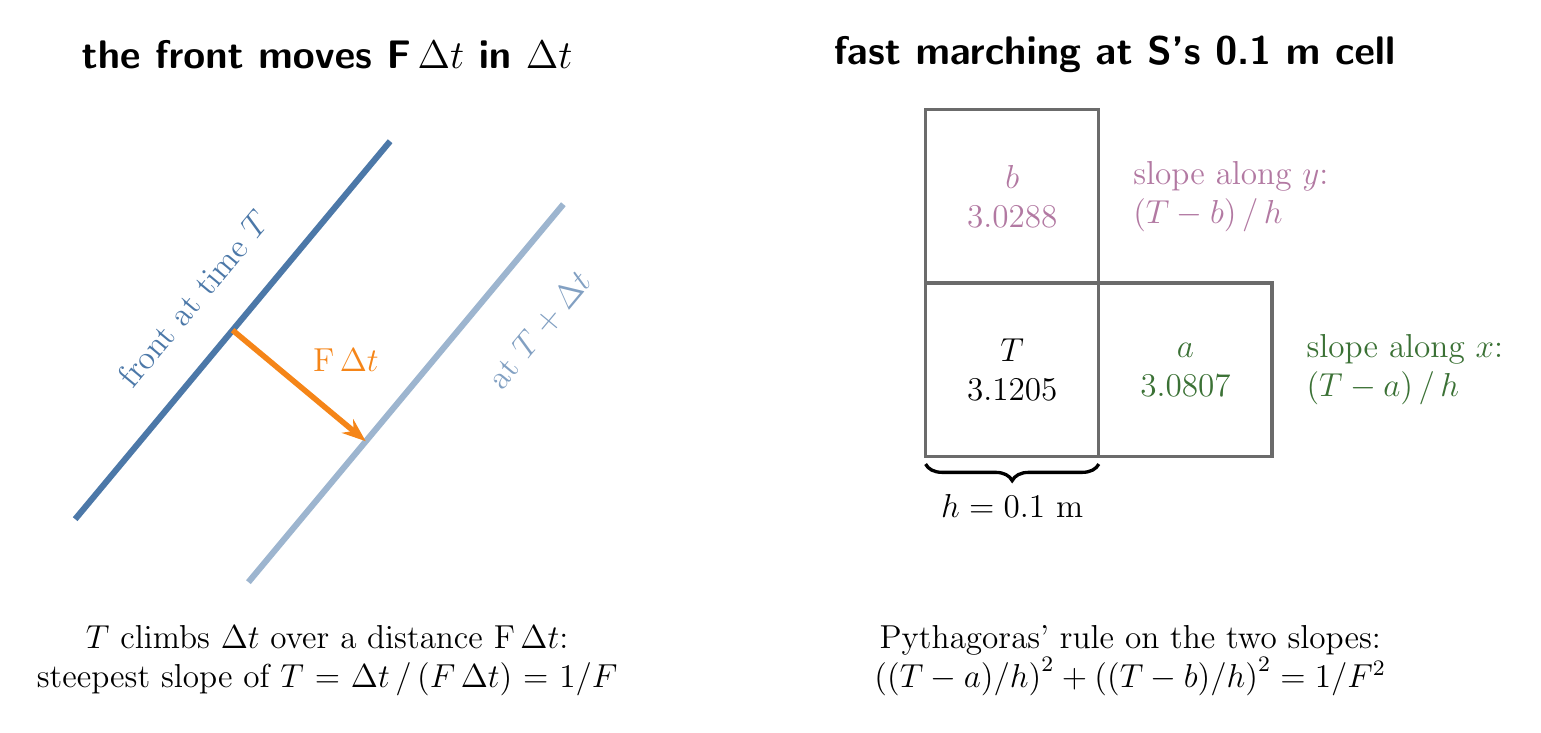
\begin{tikzpicture}[every node/.append style={font=\large}]
  % ---------- left: two fronts ----------
  \node[title] at (2.6,6.1) {the front moves F$\,\Delta t$ in $\Delta t$};
  \draw[cblue, line width=2.2pt] (-0.6,0.2) -- (3.4,5.0);
  \draw[cblue!55, line width=2.2pt] (1.6,-0.6) -- (5.6,4.2);
  \node[text=cblue, rotate=50.2] at (0.9,3.0) {front at time $T$};
  \node[text=cblue!70, rotate=50.2] at (5.3,2.6) {at $T + \Delta t$};
  \coordinate (p) at (1.4,2.6);
  \coordinate (q) at ($(p)+(1.69,-1.41)$);
  \draw[arrow, draw=corange, line width=2pt] (p) -- node[above right=1pt, text=corange] {F$\,\Delta t$} (q);
  \node[note, font=\large, text=black, align=center] at (2.6,-1.6) {$T$ climbs $\Delta t$ over a distance F$\,\Delta t$:\\
    steepest slope of $T$ $=$ $\Delta t\,/\,(\text{F}\,\Delta t)$ $=$ $1/\text{F}$};
  % ---------- right: one cell ----------
  \begin{scope}[xshift=10.2cm]
  \node[title] at (2.4,6.1) {fast marching at S's 0.1 m cell};
  \def\s{2.2}
  \draw[cgrey] (0,1) rectangle (\s,1+\s);
  \draw[cgrey] (\s,1) rectangle (2*\s,1+\s);
  \draw[cgrey] (0,1+\s) rectangle (\s,1+2*\s);
  \node[align=center] at (\s/2,1+\s/2) {$T$\\3.1205};
  \node[align=center, text=cgreen!70!black] at (1.5*\s,1+\s/2) {$a$\\3.0807};
  \node[align=center, text=cpurple] at (\s/2,1+1.5*\s) {$b$\\3.0288};
  \draw[decorate, decoration={brace, amplitude=6pt, mirror}] (0,0.9) -- node[below=7pt] {$h = 0.1$ m} (\s,0.9);
  \node[align=left, anchor=west, text=cpurple] at (\s+0.3,1+1.5*\s) {slope along $y$:\\$(T - b)\,/\,h$};
  \node[align=left, anchor=west, text=cgreen!70!black] at (2*\s+0.3,1+0.5*\s) {slope along $x$:\\$(T - a)\,/\,h$};
  \node[note, font=\large, text=black, align=center] at (2.6,-1.6) {Pythagoras' rule on the two slopes:\\
    $\big((T - a)/h\big)^2 + \big((T - b)/h\big)^2 = 1/\text{F}^2$};
  \end{scope}
\end{tikzpicture}
\end{document}
